\section{Exploratory Data Analysis \& Strategic Prescriptions}

\subsection{Data Story 1: Channel Conversion Efficiency Is Eroding While Return Risk Remains Structurally Flat}

\textbf{Descriptive.} Joining monthly \textit{web\_traffic} and \textit{orders} shows wide efficiency dispersion: social media leads at 10.40 orders per 1{,}000 sessions, while organic search records 7.39. Post-purchase quality is stable, with return rates tightly bounded between 3.33\% and 3.46\%.

\textbf{Diagnostic.} The gap is a top-of-funnel productivity problem, not a fulfillment-quality problem. High-traffic but low-yield channels (notably organic and email) depress blended media productivity despite high absolute revenue.

\textbf{Predictive.} Monthly trend slopes for \textit{orders\_per\_1k\_sessions} are negative in every channel (-0.123 to -0.093), implying rising CAC pressure if the acquisition mix remains unchanged.

\textbf{Prescriptive.} Reallocating 100{,}000 sessions from the least efficient to the most efficient channel yields +300.84 incremental orders, about +7.29 million net sales, and +0.71 million gross profit under current unit economics. Implement a weekly allocation rule: scale spend only when trailing 4-week \textit{orders\_per\_1k\_sessions} is above channel median and \textit{return\_rate} is below portfolio p75.

\begin{figure}[htbp]
\centering
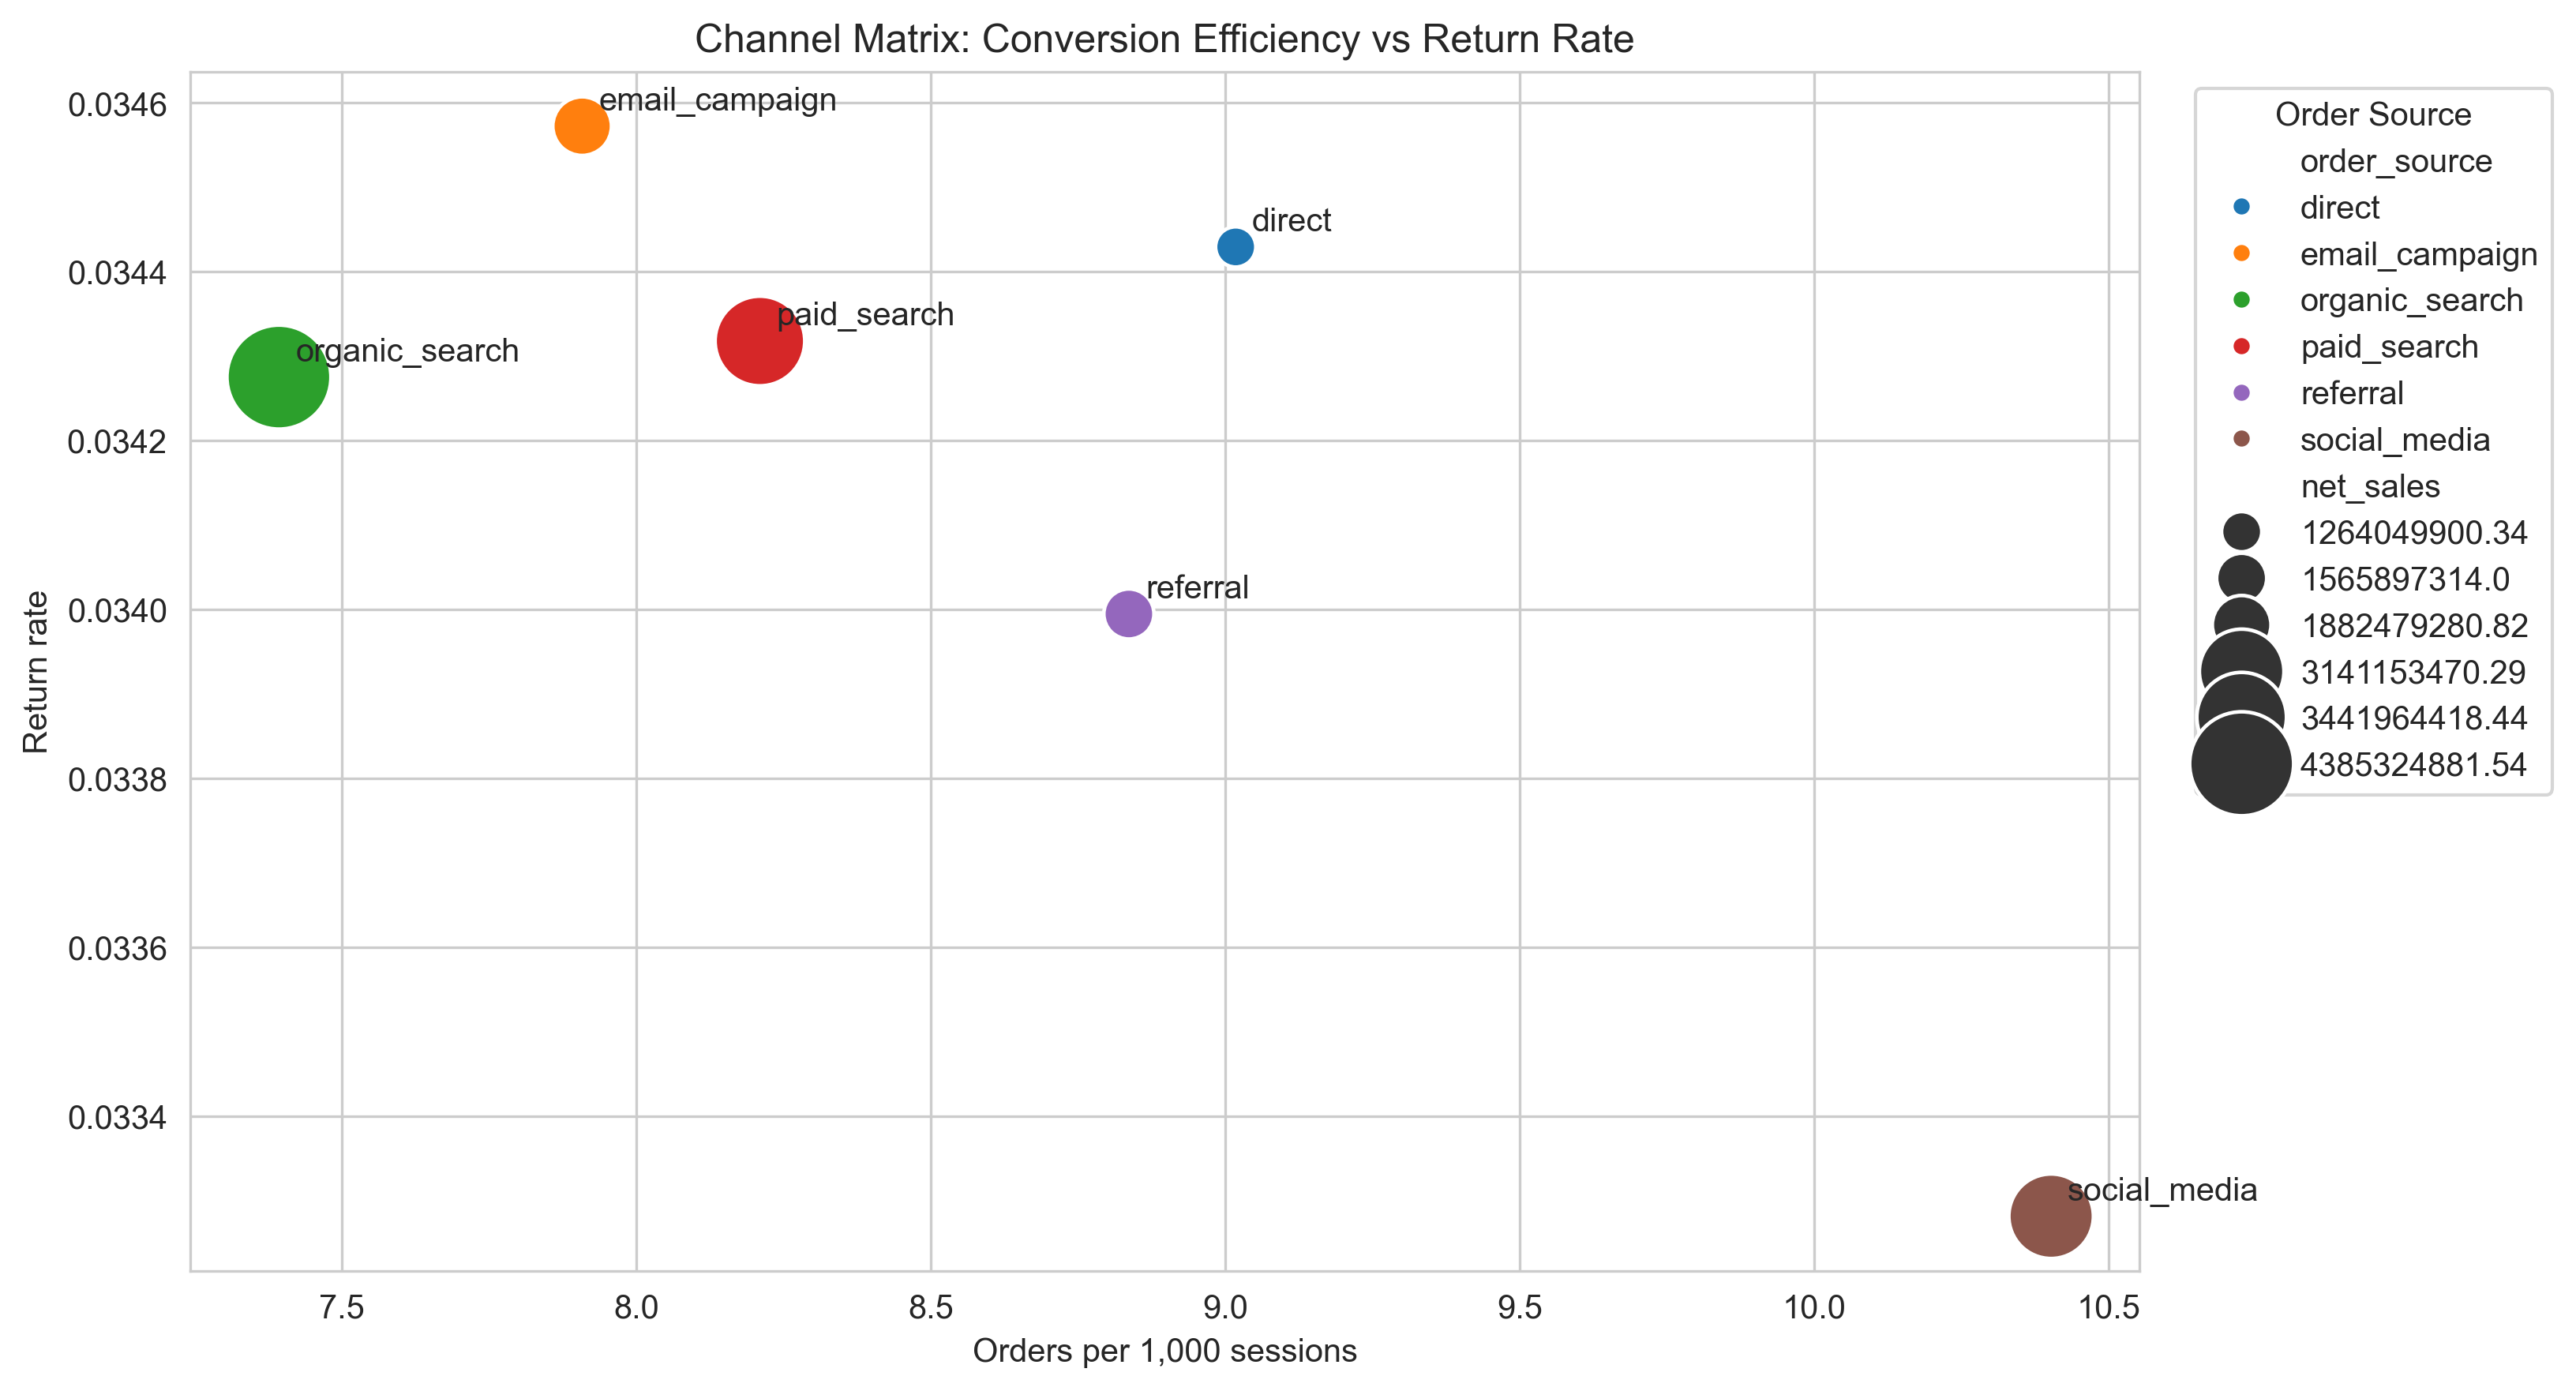
\includegraphics[width=0.8\linewidth]{figures/story1_channel_matrix.png}
\caption{\textbf{Channel Efficiency--Quality Frontier.} Bubble size denotes channel net sales; the x-axis reports conversion efficiency (orders per 1{,}000 sessions) and the y-axis reports return rate. Conversion heterogeneity is large while return risk is nearly flat, supporting short-run growth via traffic reallocation toward high-yield channels rather than quality remediation.}
\label{fig:story1_channel_matrix}
\end{figure}

\subsection{Data Story 2: Discount Intensity Beyond 10\% Systematically Destroys Gross Margin}

\textbf{Descriptive.} Margin by realized discount bucket is strongly non-linear: $\leq 5\%$ remains positive (+17.24\%), 5--10\% is near break-even (+0.87\%), while 10--20\% (-10.85\%) and $>20\%$ (-24.56\%) are negative. Promotion-type results are consistent: no-promotion +19.96\%, percentage -10.25\%, fixed-amount -63.28\%.

\textbf{Diagnostic.} The main leak is not promotion incidence itself, but deep-discount design and fixed-value mechanics that decouple markdown depth from item economics. This generates negative-contribution demand, especially when high-discount share rises in peak campaigns.

\textbf{Predictive.} If the deep-discount mix persists, high-volume campaign periods will keep compressing blended gross margin and increase earnings volatility, even with stable topline.

\textbf{Prescriptive.} Set a default markdown cap at 10\%. Permit $>10\%$ discounts only for SKUs in the top quartile of \textit{days\_of\_supply} and with non-negative projected post-discount contribution. A counterfactual re-mix shifting 20\% of net sales from $>10\%$ buckets to 5--10\% yields about +96.06 million incremental gross profit.

\begin{figure}[htbp]
\centering
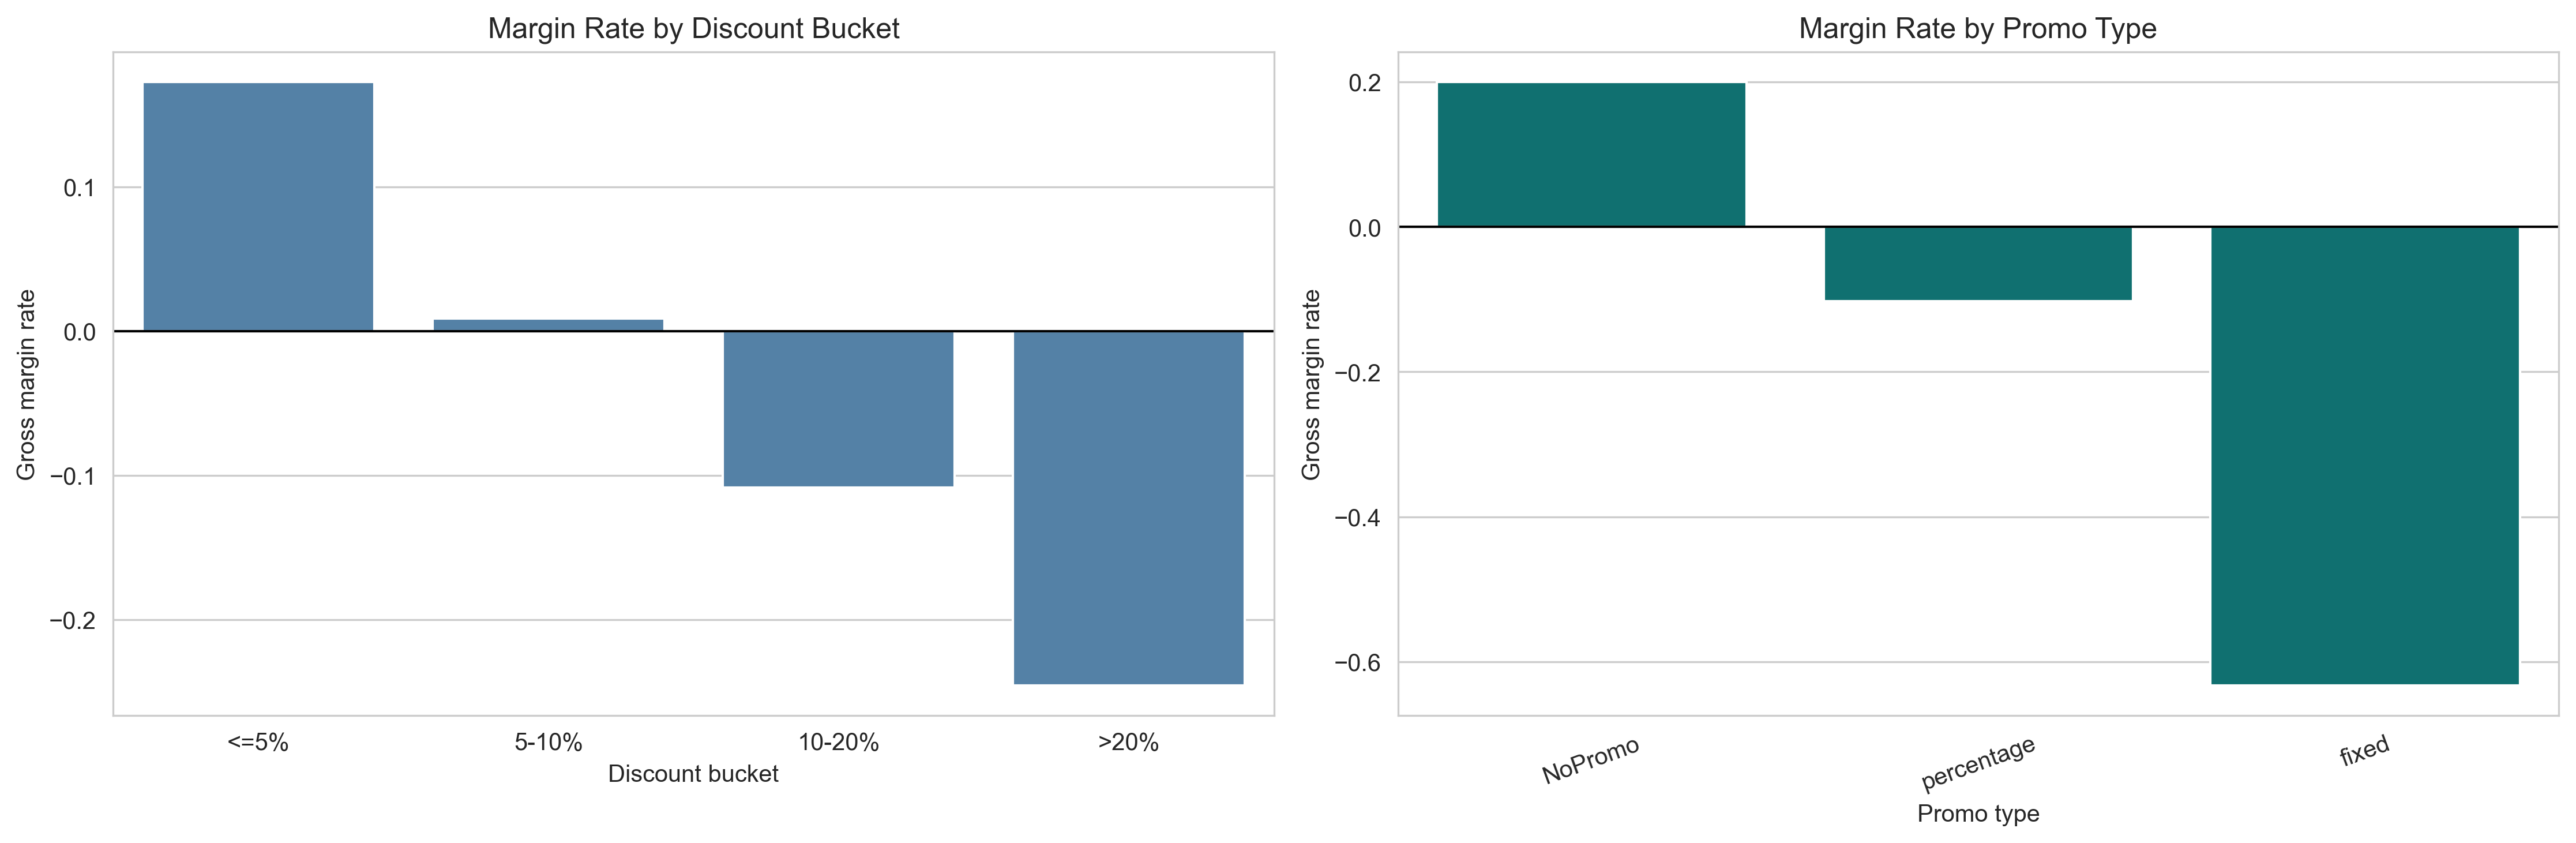
\includegraphics[width=0.8\linewidth]{figures/story2_discount_margin.png}
\caption{\textbf{Profitability Response to Discount Architecture.} The left panel reports gross margin by discount bucket; the right panel reports gross margin by promotion type. The margin sign-flip beyond 10\% and the severe underperformance of fixed-value promotions directly support discount guardrails and contribution-based campaign approval.}
\label{fig:story2_discount_margin}
\end{figure}

\subsection{Data Story 3: Joint Overstock and Refund Exposure Is Locking Working Capital}

\textbf{Descriptive.} Integrating latest inventory snapshots with category-level returns shows concentrated capital lock-in. Streetwear has the largest inventory cost (about 276.37 million), with 82.65\% overstock and a 34.89\% refund-to-gross-profit ratio. Casual has the highest refund burden relative to gross profit (41.57\%), while GenZ has the highest overstock rate (84.09\%).

\textbf{Diagnostic.} The risk reflects a two-sided operating failure: excess stock depth in slow-turn nodes and weak post-purchase retention in selected categories. Categories in the matrix upper-right simultaneously consume working capital and erode realized profitability.

\textbf{Predictive.} Without intervention, persistent overstock and refund leakage will increase cash-conversion-cycle pressure, reduce inventory agility, and crowd out reinvestment in high-velocity assortments.

\textbf{Prescriptive.} Prioritize Streetwear and GenZ for integrated liquidation-plus-quality programs with explicit margin floors. For Streetwear alone, a 10--15\% refund reduction protects 40.67--61.01 million in value; reducing locked inventory value by 5 percentage points releases about 13.82 million working capital.

\begin{figure}[htbp]
\centering
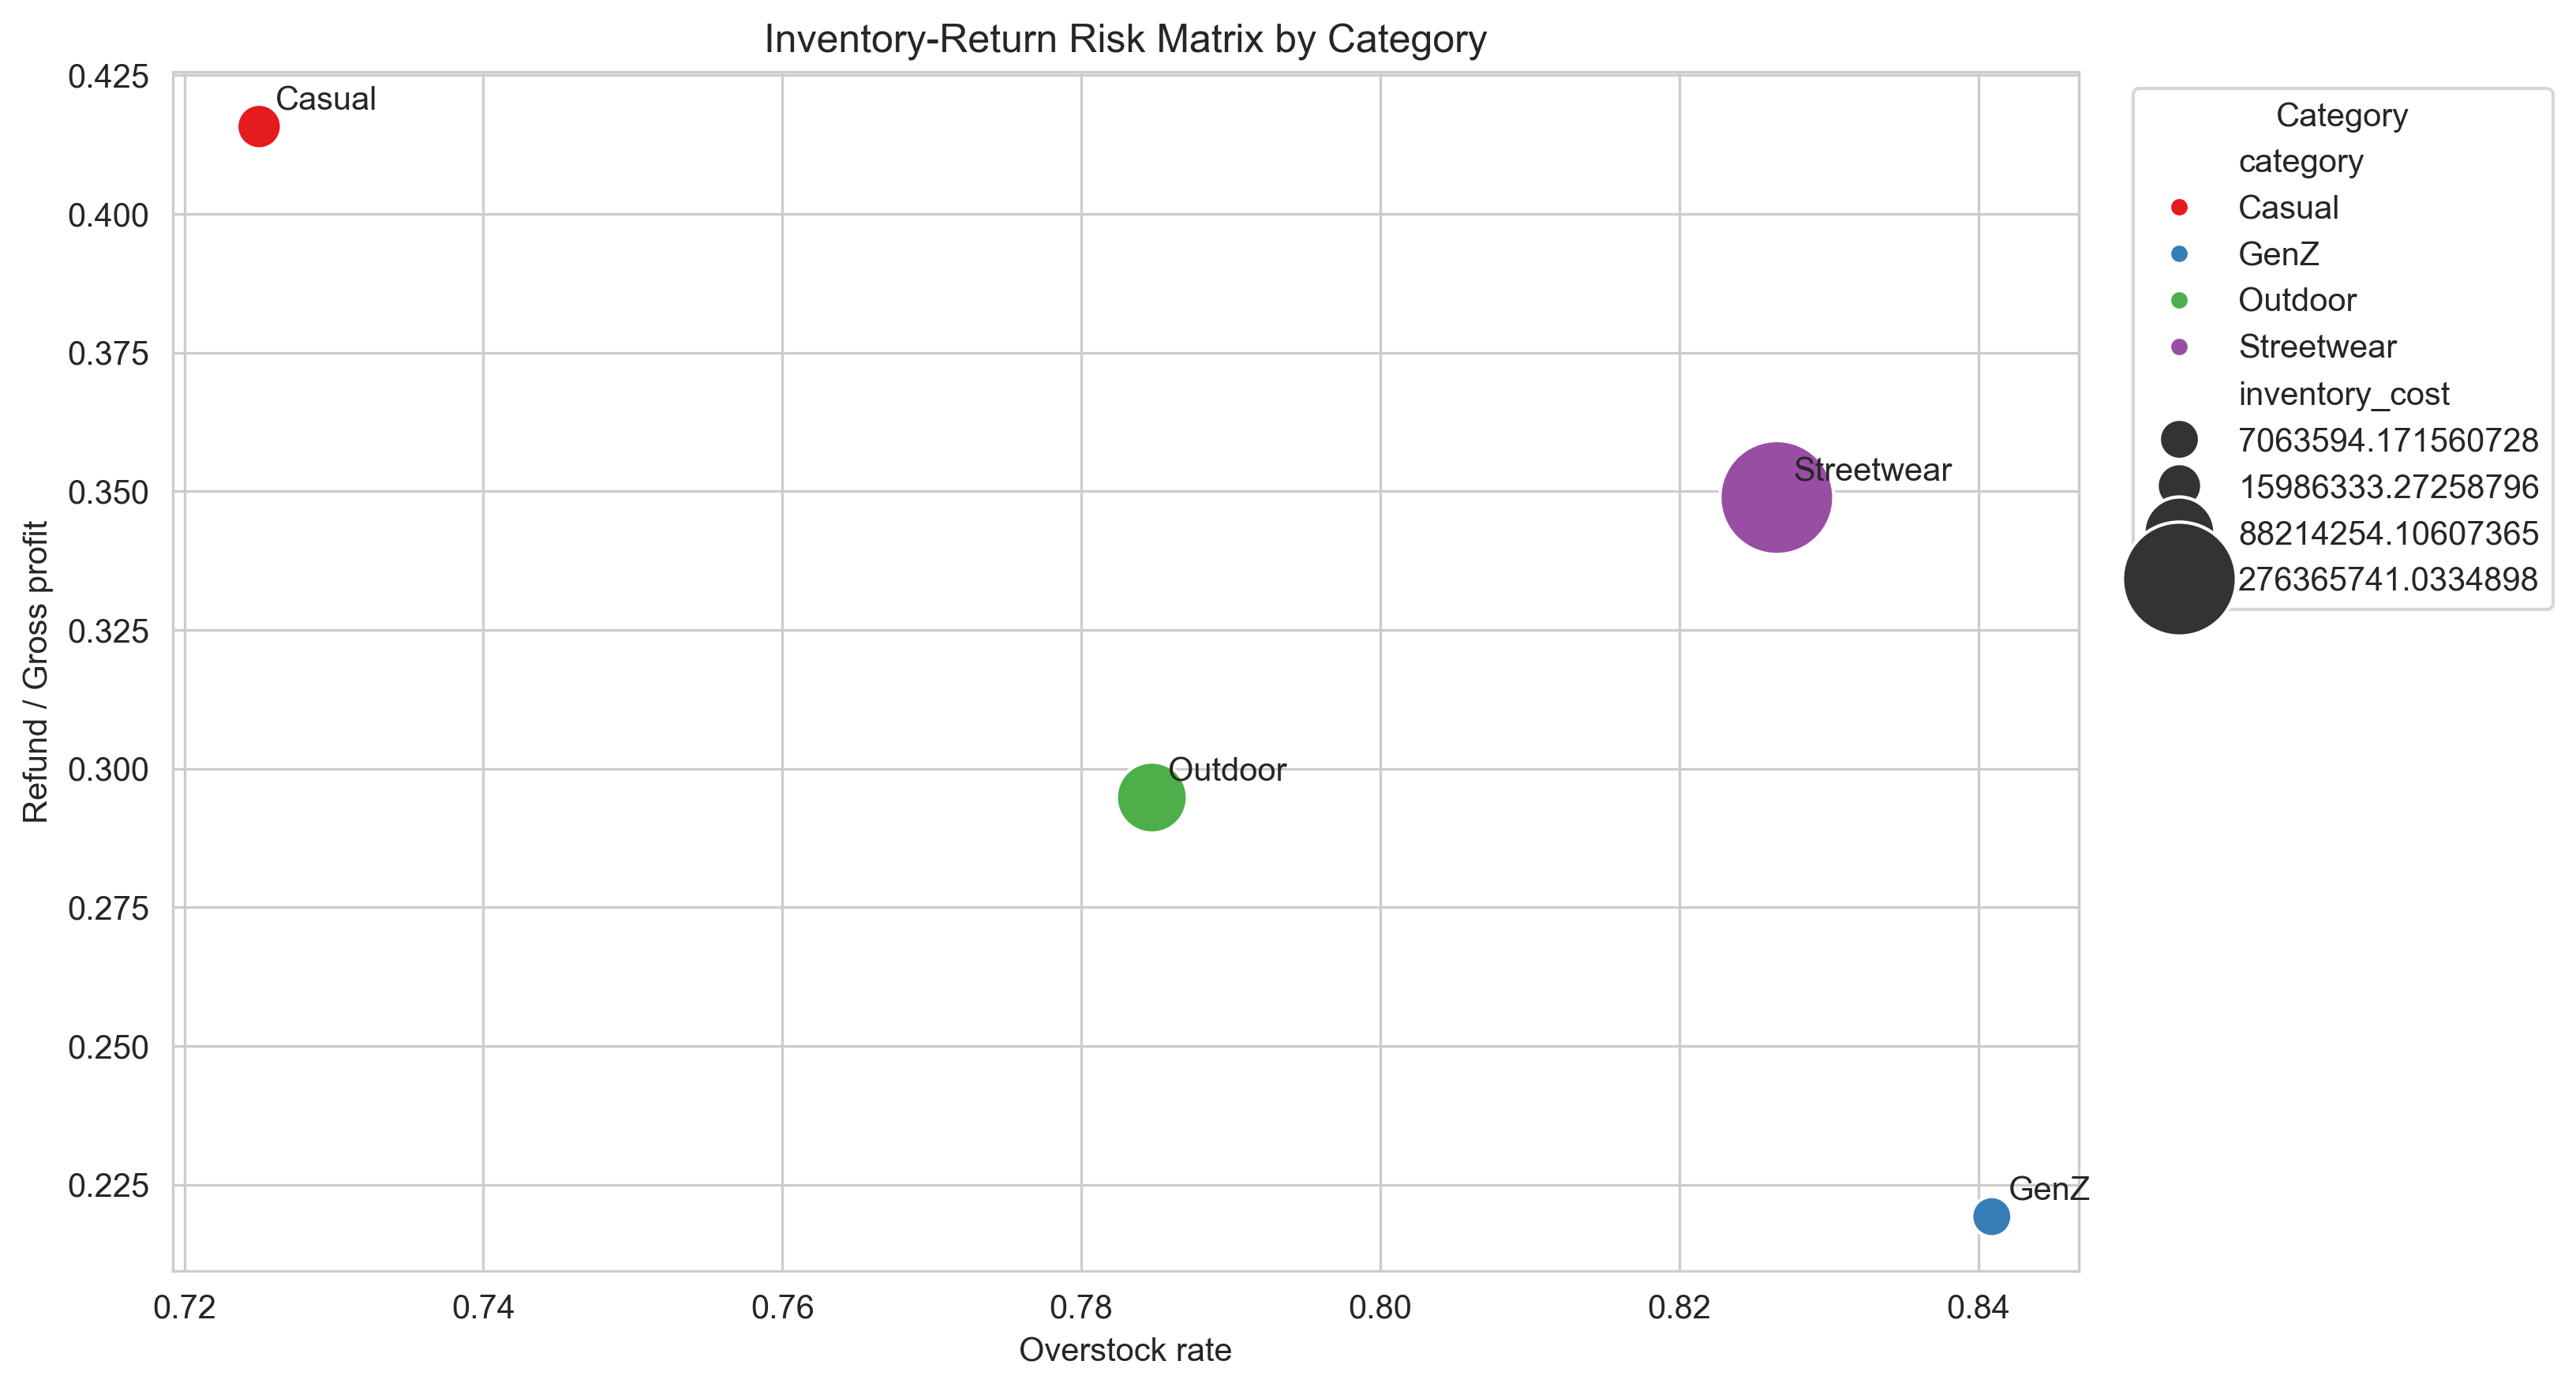
\includegraphics[width=0.8\linewidth]{figures/story3_inventory_return_risk.png}
\caption{\textbf{Inventory--Refund Risk Matrix by Category.} Bubble size encodes latest inventory cost. Categories in the upper-right quadrant combine high overstock rates with high refund-to-gross-profit ratios, signaling concurrent liquidity lock-in and profit leakage. The plot isolates where coordinated pricing, inventory normalization, and return mitigation produce the largest near-term financial impact.}
\label{fig:story3_inventory_return_risk}
\end{figure}

\subsection{Executive Synthesis}
Across all three stories, the optimization axis is not revenue at any cost, but contribution-quality growth under capital discipline along \textit{Channel $\times$ Discount Depth $\times$ Inventory Risk}. We recommend a weekly control-tower tracking five KPIs: \textit{orders\_per\_1k\_sessions}, \textit{gross\_margin\_rate}, \textit{return\_rate}, \textit{overstock\_rate}, and \textit{refund\_to\_gp}, with explicit trigger thresholds linked to budget, markdown, and replenishment decisions.
